\subsection{Display Worker}\label{sec:display-worker}

The display-worker is responsible for showing content to users on whatever screen
that they are using. This component must be able to adapt to a variety of different
environments, be it the 360 degree panoramic screen, a wall of giant monitors, or 
just a user's desktop machine. Additionally, we aim to have something capable of 
showing a variety of content, both developed in-house as well as arbitrary 
third-party content, allowing for a larger variety of use-cases and usage than
some previous art, where all content had to be built for their environment.

\begin{figure}
    \centering
    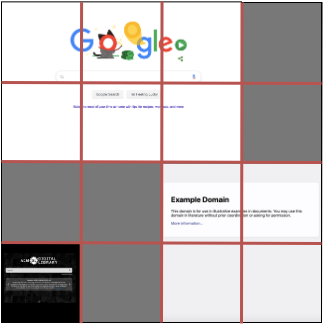
\includegraphics[width=0.5\columnwidth]{chapters/02_technology/figures/display_server.png}
    \caption{Diagram highlighting the grid of the display-worker. The red lines are added here for clarity, and are not present in the actual software.}
    \label{fig:display_server_grid}
\end{figure}

To accomplish this, we build off the open-source 
Electron~\footnote{https://www.electronjs.org/} application, which provides a
wrapper around the Chromium project to build desktop applications. Through this,
our content then is displayed as websites within the display-worker, where the 
websites can be pointing at localhost applications, or external sites. The 
display-worker is set-up such that it provides the user with a N by M grid, where
N and M are configurable beforehand to fit the environment, where a user may open
any number of webviews to take up X by Y rectangle on the grid. Within each
webview, we load a website. Webviews may stack upon each other, and be moved as 
needed by a user. An example of this is shown in 
Figure~\ref{fig:display_server_grid}. When dealing with multiple displays, we
assume that the displays are ``continuous'', and share the same dimensions as
all other displays within the grid. The grid is then divided equally amongst all 
screens.

Manipulating the webviews, be it opening or closing them, moving them around,
or resizing the amount of cells it takes up can be done utilizing RabbitMQ,
wherein a JSON message is passed to describe the change. When opening a
webview, the JSON message contains additional parameters that describe
capabilities of the webview. For example, this may include option saying that
the webview can be zoomed into and out of or that it is MUIFOLD
compatible (described more below). All changes in webviews is broadcast from
the display-worker, which can be utilized by other systems.

Separate for the webviews, the display-worker exposes an additional RabbitMQ
endpoint which is used for displaying the cursor. Through this topic, each
message contains a cursor id, the x,y location on where to show the cursor
and the type of cursor to show, which includes an open hand which is the
default state and a closed hand to symbolize clicking on or scrolling content.